\documentclass{article}

% ------------------------------------ %
%             Document Info            %
% ------------------------------------ %

\usepackage{../../../LaTeX-Preamables/Assign}

\begin{document}
\newcommand{\documentcourse}{ENGG1300}
\newcommand{\documentnumber}{4}

% ------------------------------------ %
%                Header                %
% ------------------------------------ %

\begin{minipage}{0.07\textwidth}
    
\includegraphics[width=\linewidth]{../../../LaTeX-Preamables/LaTeX-Templates/HKULOGO256.png}
\end{minipage}
\hspace{0.02\textwidth}
\begin{minipage}{0.55\textwidth}
    \documentcourse

    Assignment \documentnumber

    SID: 3036268218
\end{minipage}
\begin{minipage}{0.35\textwidth}
    \begin{flushright}
        Jax

        \jobname.pdf

        \today
    \end{flushright}
\end{minipage}

\vspace{0.5cm}

\hrule

% ------------------------------------ %
%                Content               %
% ------------------------------------ %
\centering
\section*{Question 1}
\subsection*{Question 1a}
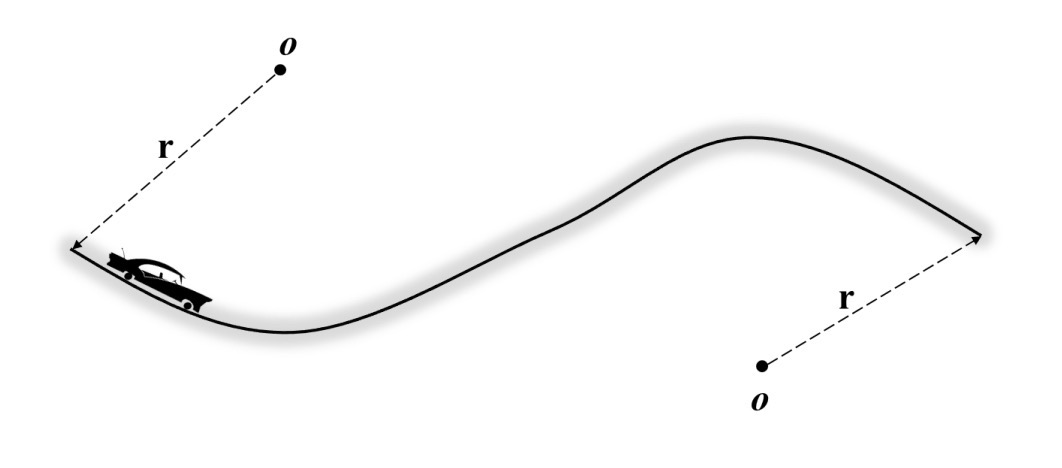
\includegraphics[width=0.5\textwidth]{img/A4Fig1.jpg}

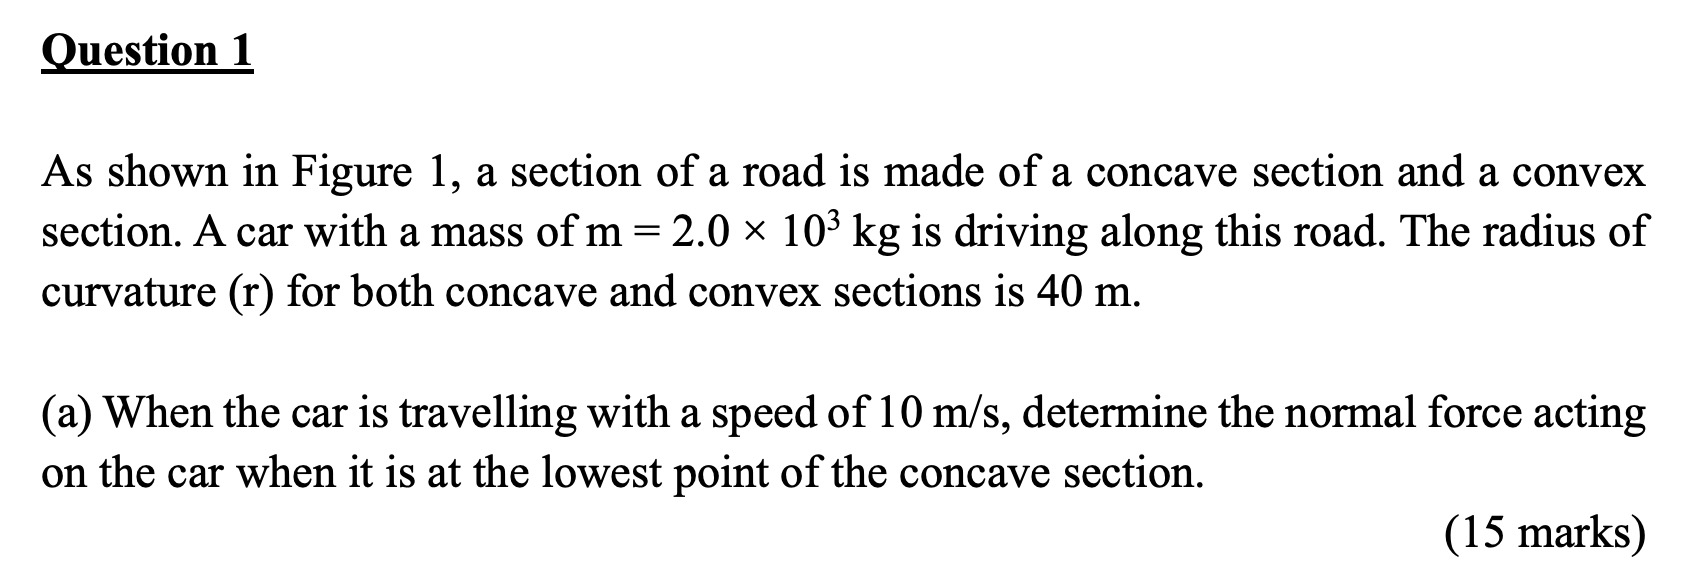
\includegraphics[width=0.7\textwidth]{img/A4Q1a.jpg}
\begin{align*}
    v_i & = 10\ ms^{-1}            \\
    a_c & = \frac{v_i^2}{r}        \\
        & = \frac{10^2}{40}        \\
        & = 2.5\ ms^{-2}           \\
    N   & = m(g + a_c)             \\
        & = 2\times10^3(9.8 + 2.5) \\
        & = 24.6\ kN               \\
\end{align*}
\subsection*{Question 1b}
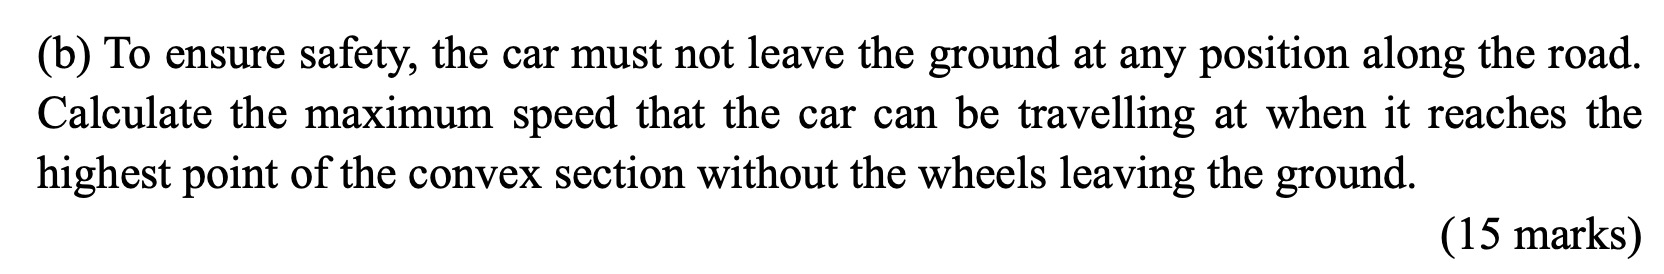
\includegraphics[width=0.7\textwidth]{img/A4Q1b.jpg}
\begin{align*}
    mg               & = ma_c          \\
    g                & = a_c           \\
    \frac{v_i^2}{40} & = 9.8           \\
    v_i              & = 19.8\ ms^{-1} \\
\end{align*}

\section*{Question 2}
\subsection*{Question 2a}
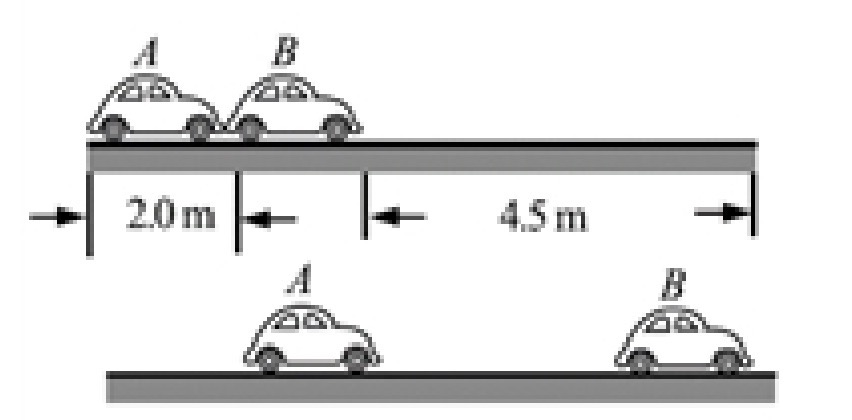
\includegraphics[width=0.5\textwidth]{img/A4Fig2.jpg}

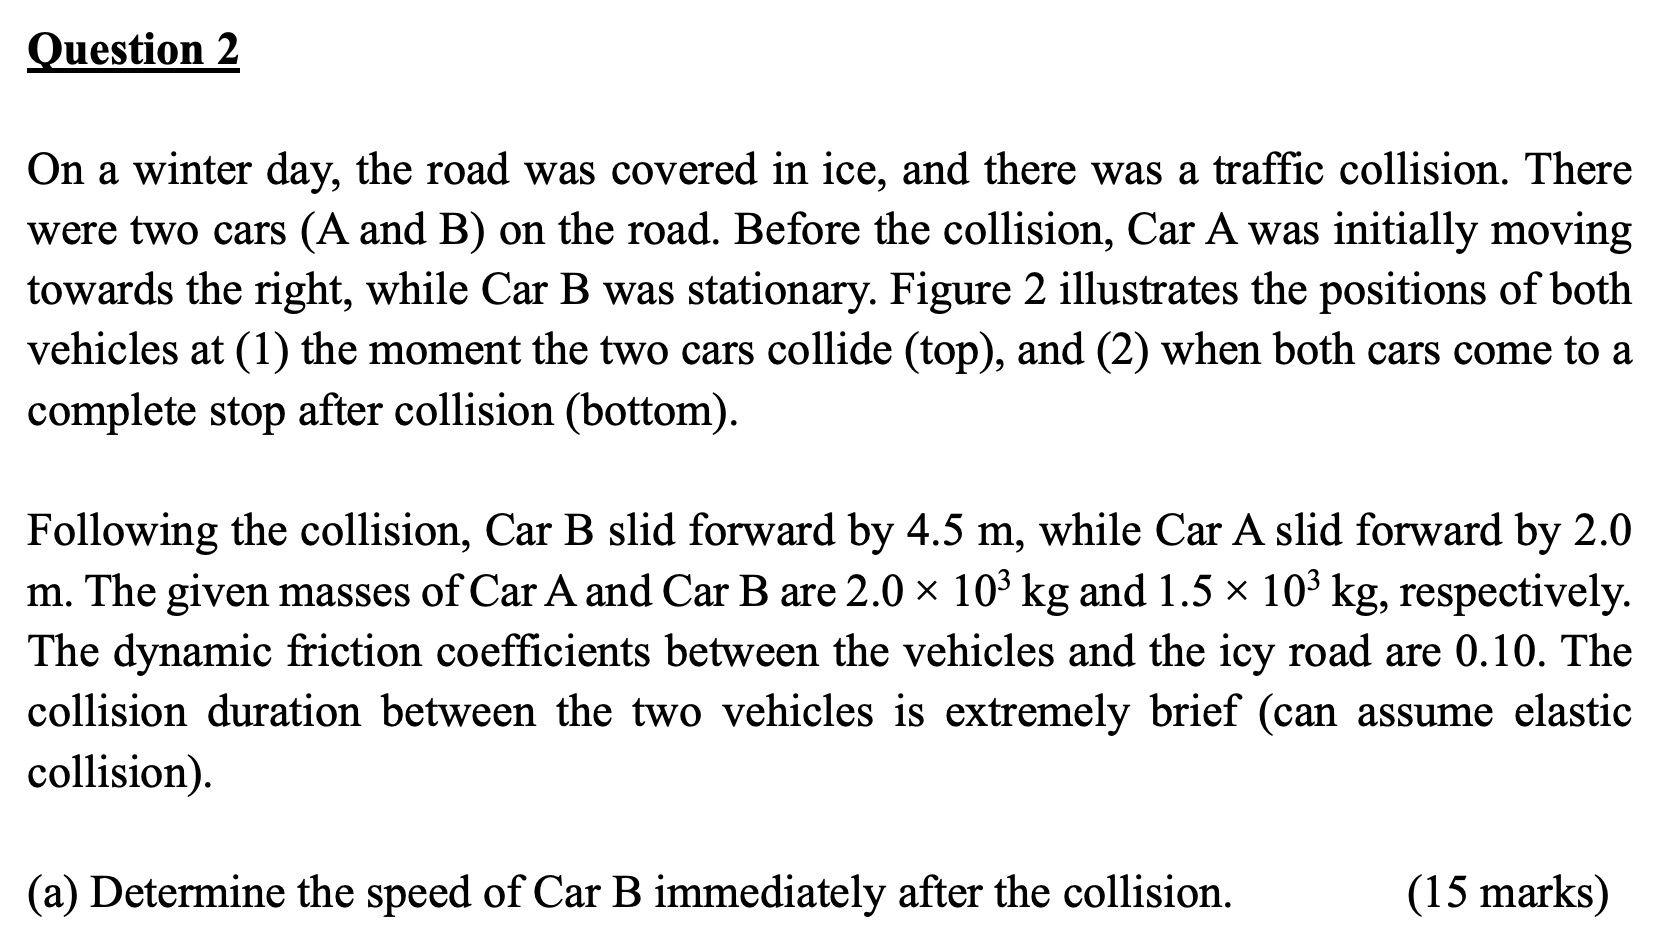
\includegraphics[width=0.7\textwidth]{img/A4Q2a.jpg}
\begin{align*}
    v_B^2 & = u_B^2 + 2as                         \\
    u_B^2 & = v_B^2 - 2as                         \\
    u_B   & = \sqrt{-2as}                         \\
          & = \sqrt{2\mu gs}                      \\
          & = \sqrt{2\times0.1\times9.8\times4.5} \\
          & = 2.97\ ms^{-1}                       \\
\end{align*}
\subsection*{Question 2b}
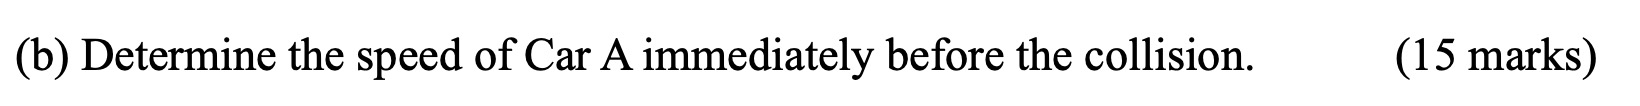
\includegraphics[width=0.7\textwidth]{img/A4Q2b.jpg}
\begin{align*}
    v_A^2        & = u_A^2 + 2as                                                     \\
    u_A^2        & = v_A^2 - 2as                                                     \\
    u_A          & = \sqrt{-2as}                                                     \\
                 & = \sqrt{2\mu gs}                                                  \\
                 & = \sqrt{2\times0.1\times9.8\times2}                               \\
                 & = 1.98\ ms^{-1}                                                   \\
    m_{A0}v_{A0} & = m_{A1}v_{A1} + m_{B1}v_{B1}                                     \\
    v_{A0}       & = \frac{2\times10^3\cdot1.98+1.5\times10^3\cdot2.97}{2\times10^3} \\
                 & = 4.21\ ms^{-1}                                                   \\
\end{align*}

\section*{Question 3}
\subsection*{Question 3a}
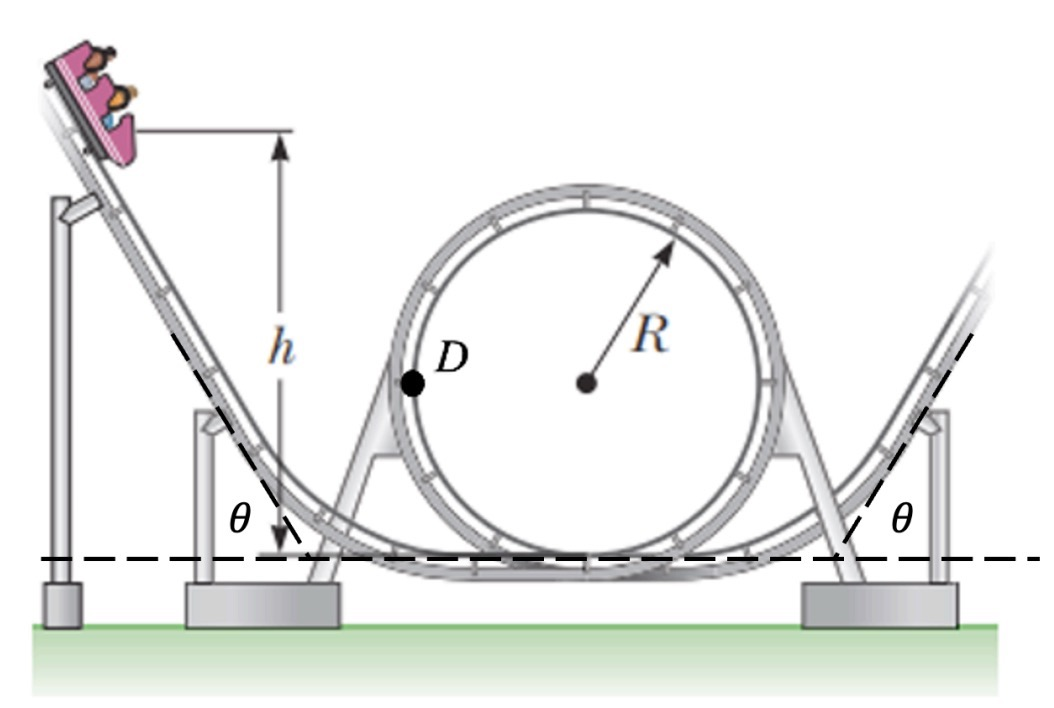
\includegraphics[width=0.5\textwidth]{img/A4Fig3.jpg}

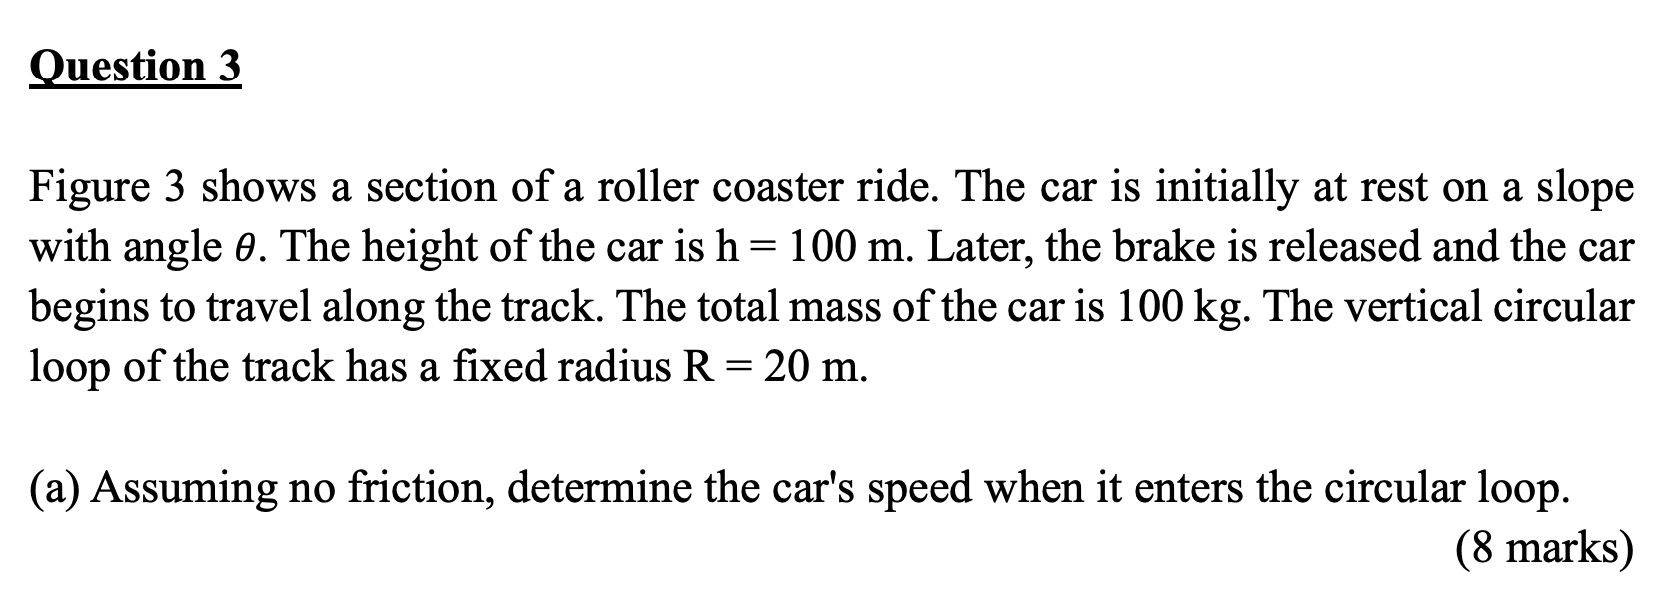
\includegraphics[width=0.7\textwidth]{img/A4Q3a.jpg}
\begin{align*}
    E_{GP}       & = E_k               \\
    mgh          & = \frac{1}{2}mv^2   \\
    gh           & = \frac12v^2        \\
    9.8\times100 & = \frac12\times v^2 \\
    v            & = 44.3\ ms^{-1}     \\
\end{align*}
\subsection*{Question 3b}
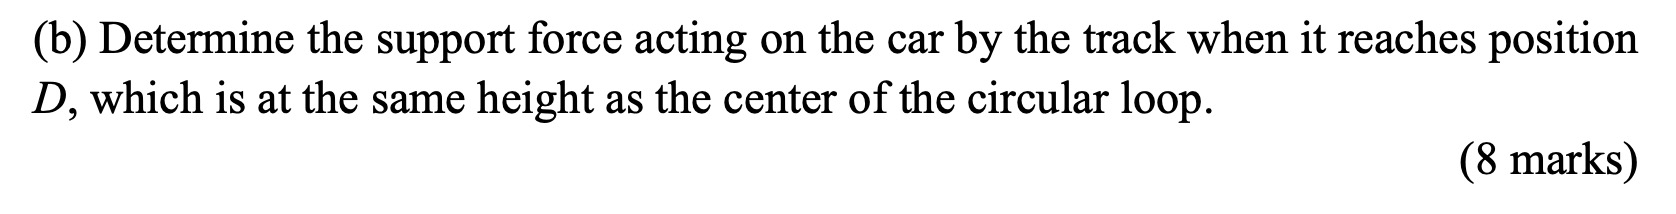
\includegraphics[width=0.7\textwidth]{img/A4Q3b.jpg}

The support force that the track exerts on the car is the normal force.
\begin{align*}
    N & = F_c                        \\
      & = \frac{mv^2}{r}             \\
      & = \frac{100\times44.3^2}{20} \\
      & = 9.81\ kN                   \\
\end{align*}
\subsection*{Question 3c}
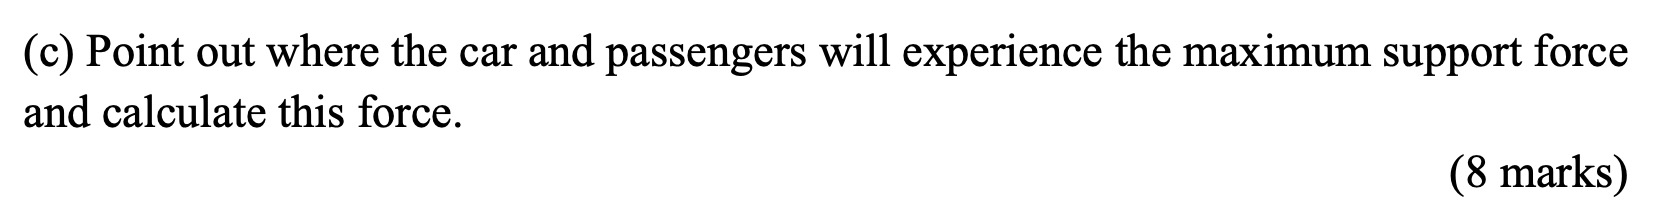
\includegraphics[width=0.7\textwidth]{img/A4Q3c.jpg}

The maximum normal force occurs at the bottom of the loop.
\begin{align*}
    N & = m(g + a_c)                   \\
      & = 100(9.8 + \frac{v^2}{r})     \\
      & = 100(9.8 + \frac{44.3^2}{20}) \\
      & = 10.8\ kN                     \\
\end{align*}
\subsection*{Question 3d}
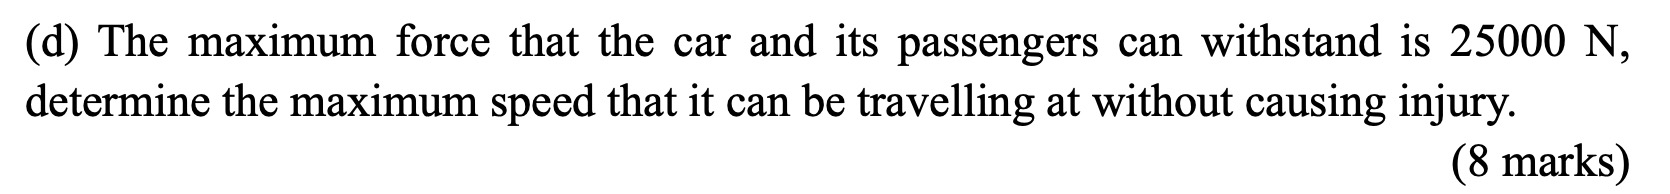
\includegraphics[width=0.7\textwidth]{img/A4Q3d.jpg}
\begin{align*}
    N     & \le m(g + \frac{v^2}{r})      \\
    25000 & \le 100(9.8 + \frac{v^2}{20}) \\
    v     & \le 69.3\ ms^{-1}             \\
\end{align*}
\subsection*{Question 3e}
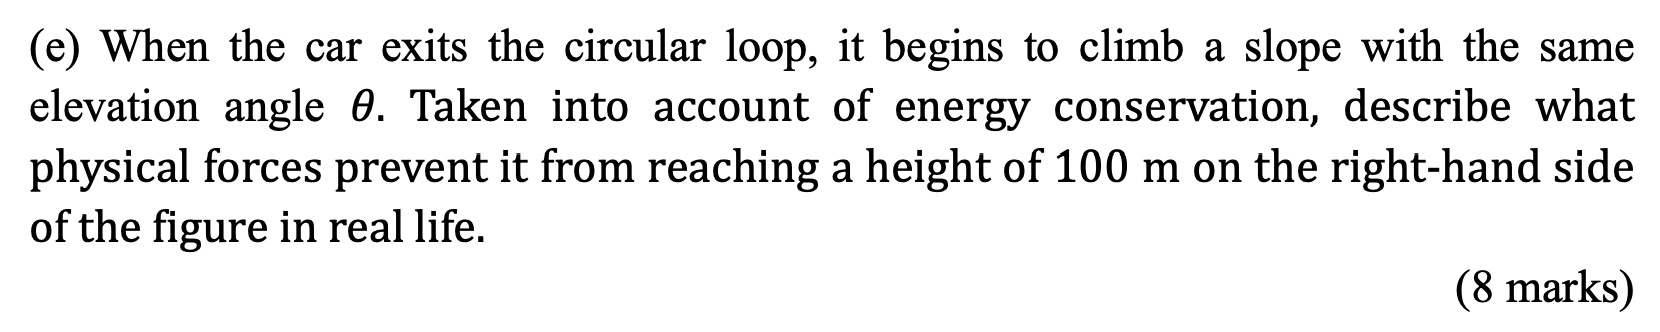
\includegraphics[width=0.7\textwidth]{img/A4Q3e.jpg}

The car is able to reach the same height as the initial on the right-hand side if all energy is conserved. However, in real life, energy can be lost due to the following physical forces:
\begin{itemize}
    \item Friction between the wheels and the track
    \item Air resistance
\end{itemize}
The lost energy is transferred to heat and sound.

\end{document}